\documentclass[authoryear, 12pt,5p, times]{elsarticle}
%\usepackage[hypcap]{caption}
%\geometry{margin=0.95in,top=1.4in,bottom=1.4in}
\geometry{margin=1.1in,top=1.5in,bottom=1.5in}
\usepackage{float}
\usepackage{amsmath}
\usepackage[hidelinks]{hyperref} 
 \usepackage{gensymb}
\usepackage{subcaption}
\usepackage{url}
%\renewcommand\thefootnote{\fnsymbol{\dagger}}
\usepackage[symbol*]{footmisc}
\makeatletter
\newcommand{\rpm}{\raisebox{.3ex}{$\scriptstyle\pm$}}
\begin{document}
\begin{frontmatter}
\title{Semiconductor Diodes}
\author{\today \quad \\Jung Lin (Doris) Lee [Lab Partner: Leah Tom]\\Prof. William Holzapfel, GSI Thomas Darlington, Thomas Mittiga, John Groh,  \\Victoria Xu, Jonathan Ma, Francisco Monsalve, Xiaofei Zhou}
	 
\end{frontmatter} 

\section*{Introduction\label{intro}}
\section{Diodes}
\section*{3.1}
We connected the 1N4448 diode to the DMM in one direction and measured a resistance of 0.61572$k\Omega$ $\pm$ 0.1138864 $\Omega$. When we reversed direction of the diode and connected the positive grabber to the black band of the diode (Cathode) and the grounding grabber to the red end of the diode(anode), the DMM measured resistance overload. 
\par This shows that diode conducts only unidirectionally, since if there is a non-overloading resistance reading, it means that the tiny test current passed by the DMM actually pass through to the other end of the terminal, resulting in a forward voltage drop across the diode.
\footnote{The minigabbers and BNC cable were connected to the INPUT pairs on the right which had a diode symbol below it.}
\section*{3.2}
In the conducting direction, the plastic-stick mounted 1NN4448 diode has a forward voltage drop of 4.419 mV$\pm$ 4.53$\mu$V.  When we squeezed the diode with our fingers, the measured forward voltage drop is 8.215.
When we submerged the diode in liquid nitrogen ---
Squeezing the diode with our finger causes slight temperature increase in the diode. We can clearly see the increasing trend of ----- as the we change the temperature of the diode.
\par Diodes do not follow the linear Ohmic behaviour relating voltage and current, but these results still correspond to the semiconductor physics at play. As we decrease the temperature, the conduction electrons has less kinetic energy and therefore slower thermal velocities. Therefore, it requires more work to transport them through the pn junction, since voltage is work per change, the results in a higher voltage drop measured. 
\section*{3.3}
We connect the offset adder to the DMM to measure the output voltage and variaed it from -8 to 8 V. Turning the knob clockwise increases the voltage and vice versa for counterclosewise. We loaded up different resistors 
\section*{3.4}
\begin{figure}[h!]
\center
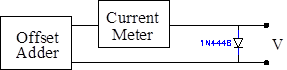
\includegraphics[width=0.5\textwidth]{figure/3_4_diag}
\caption{Setup for }
\label{3_4_diag}
\end{figure}
\section*{3.5}
The curver tracer is  

\par We rearrange the diode equation as shown in Eq. \ref{diode_eq} and solve for n as in Eq.\ref{n}
\begin{equation}
i(V) = i_{sat}\Bigg[exp(\frac{eV}{nkT})-1\Bigg]
\label{diode_eq}
\end{equation}
\begin{equation}
\begin{split}
n &= \frac{eV}{kT}\frac{1}{ln[\frac{i(V)}{i_{sat}}+1]} \\&= \frac{(1.60\times10^{-19}C)(0.368V)}{1.38\times10^{-23}m^2kgs^{-2}K^{-1}(298K)ln(\frac{0.015A}{5.22\times10^{-7}}+1)}
\label{n}
\end{split}
\end{equation}



we do indeed find that the constant n fall within the reasonable range of 1~ 2  depending on the particular diode.
\section*{3.6}
We setup the experiment by connecting the 1N4448 diode in series with a 1M$\Omega$ resistor and a 12V voltage supply. In order to find the current thoruhg the diode, we measure the value of the voltage drop across the resistor as 327 mV. Using the diode equation (Eq.\ref{diode_eq}), we compute the current through the diode, i(V=327mV), as: 
\begin{equation*}
(4.00\times10^{-8}A)e^{\frac{(1.6\times10^{-19}C)(327\times10^{-3}V)}{(1.4315)(1.38\times10^{-23}m^2kgs^{-2}K^{-1})(298K)}}
\end{equation*}
and obtain current value of 0.2896 mA.
\section*{3.7}\label{3_7_q}
We built a half wave rectifier using the setup shown in Fig.\ref{3_7_setup} and set the DC offset as zero. 
\begin{figure}[h!]
\center
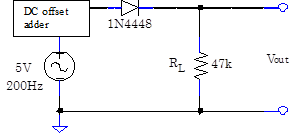
\includegraphics[width=0.5\textwidth]{figure/3_7_setup}
\caption{ setup}
\label{3_7_setup}
\end{figure}
By measuring the input and output signal waveforms, as shown in Fig.\ref{3_7_trace}, we find that the peak-to-peak voltage of the rectified signal is attenuated by a factor of about 8. In addition, we can see that the half-wave rectifier passes half of the signal while blocking the other half, however, there are still some rippling in the rectified signal that requires filtering.
\begin{figure}[h!]
\center
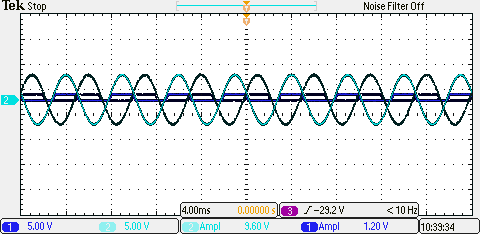
\includegraphics[width=0.5\textwidth]{figure/3_7}
\caption{Scope trace of the AC signal (in cyan; Channel 2) and the rectified output signal (in blue; Channel 1)}
\label{3_7_trace}
\end{figure}
\section*{3.8}
To alleviate the rippling effect observed in Fig.\ref{3_7}, we add a 1$\mu$F capacitor in parallel to the load resistor in the rectifier shown in Fig.\ref{3_7_setup}.

When we double the input frequency, the amplitude of the ripple -----. Doubling the capacitance results in ------. By doubling the load resistor, -------.
\section*{3.13}
When we flipped the polarity of the power supply, the forward voltage drop is close to zero because no current should be flowing through in the reverse direction of a diode. When we connected the LED to different values of resistance, we find that as we increase the resistance, the forward voltage drop increases and the LED brightness dims. When the resistance too large, the voltage drop across the diode is not enough to power the LED since it is below the LED's cutoff voltage, therefore the LED did not light up for the $30k\Omega$ and 300k$\Omega$ trial.
\begin{figure}[h!]
\center
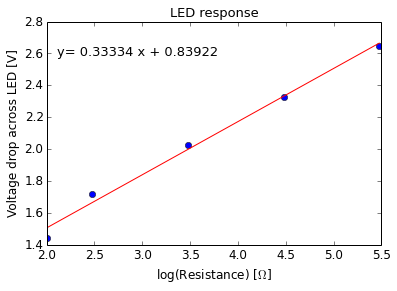
\includegraphics[width=0.5\textwidth]{figure/3_13_LED}
\caption{The LED's brightness decreases as we increase the resistance, corresponding to a larger voltage drop across the resistance.}
\label{3_13_LED}
\end{figure}
\section{Conclusion}
\section*{Acknowledgments}
\begin{footnotesize}
The author would like to acknowledge support from the GSI in this lab and with the handling of liquid nitrogen. I would also like to thank my partner, Leah Tom, for helpful discussion and collaboration that helped this work. We also appreciate Sissi Wang for providing us with guidance on question 3.2.
\end{footnotesize}
  \section*{References}
 \begin{footnotesize}
 \begin{itemize}
 \item Horowitz, Paul, and Winfield Hill. \textit{The Art of Electronics}. Cambridge: Cambridge UP, 1989. Print.
 \item ``Lab 1 - Introductory Experiments and Linear Circuits I." \textit{Donald A. Glaser Advanced Lab.} Regents of the University of California, n.d. Web. 01 Feb. 2015.
  \item ``Writing Lab Reports." \textit{Donald A. Glaser Advanced Lab.} Regents of the University of California, n.d. Web. 01 Feb. 2015.
% \item Press, William H., and William T. Vetterling. \textit{Numerical Recipes in C: The Art of Scientific Computing}. Cambridge University Press, 1992.  
\end{itemize}
% \bibliography{references}
%\bibliographystyle{elsarticle-harv}
  \end{footnotesize}

\end{document}
